\section{H-Bridge}
The H-bridge see \figref{Hbridge} is a commonly used circuit for motor control. To control the motor some FET(s) are controlled with a PWM signal. The duty cycle of this PWM signal determines at which velocity the motor will run.

\begin{figure}[H]
	\centering
	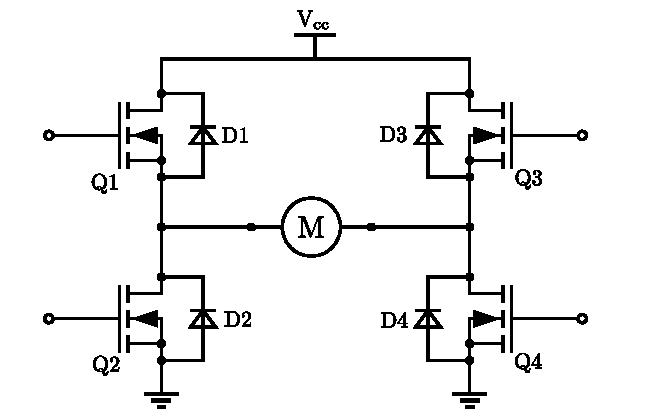
\includegraphics[scale=.6]{figures/Hbridge.pdf}
	\caption{Standard H-bridge}
	\label{Hbridge}
\end{figure}

There exists a wide range of configurations in which the H-bridge can be implemented. These configurations determines the modes of operation, where each mode has some different properties. Some of the common modes are described in the following sections.

\subsection{Regenerative Coast Mode}
One mode of operation is the coast mode, where the PWM signal controls 2 of the 4 FETs, Q1 and Q3, as seen on \figref{HbridgeClockwiseCoastON}. In the on-period of the PWM signal the Q1 and Q4 are turned on, leading the current from Vcc through the motor and down to ground. This means that the motor is driven by the supply when the PWM goes high. When the PWM goes low, both Q1 and Q4 are shut off. Given that Q2 and Q3 are permanently off, the current generated by the motor in its armature will be driven through the intrinsic diodes of Q2 and Q3. So when the PWM goes low, the battery is charged.

  \begin{minipage}{\linewidth}
  	\centering
  	\begin{minipage}{0.45\linewidth}
  		\begin{figure}[H]
  			\centering
  			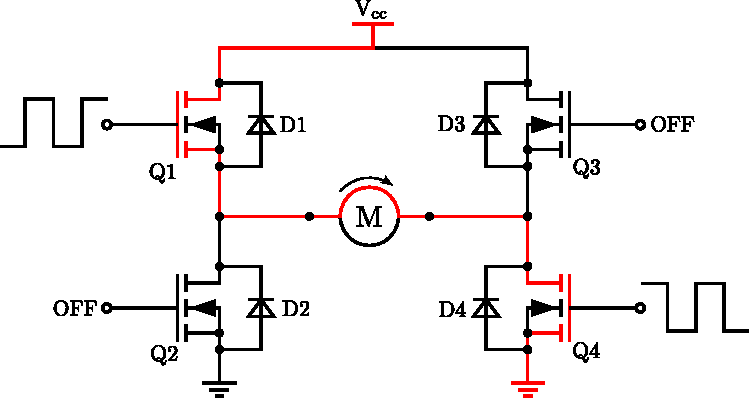
\includegraphics[scale=.6]{figures/HbridgeClockwiseCoastON.pdf}
  			\caption{Clockwise coast operation in on-state}
  			\label{figures/HbridgeClokwiseCoastON}
  		\end{figure}
  	\end{minipage}
  	\hspace{0.03\linewidth}
  	\begin{minipage}{0.45\linewidth}
  		\begin{figure}[H]
  			\centering
  			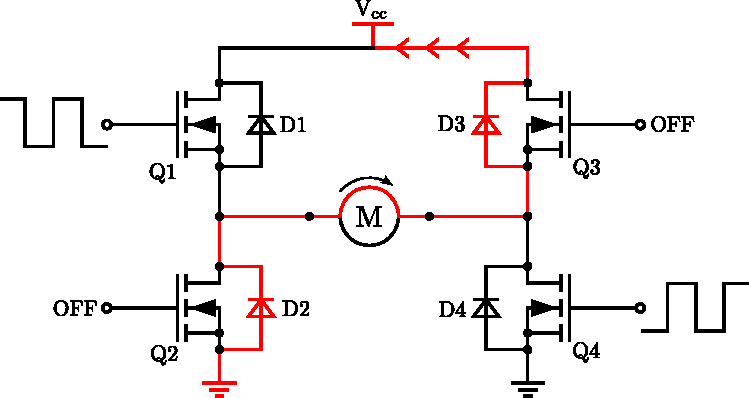
\includegraphics[scale=.6]{figures/HbridgeClockwiseCoastRegen.pdf}
  			\caption{Clockwise coast operation in off-state}
  			\label{HbridgeClokwiseCoastRegen}
  		\end{figure}
  	\end{minipage}
  \end{minipage}

\subsection{4Q Mode}
In this mode of operation the PWM signal is imposed on all 4 FETs, as seen on \figref{HbridgeClokwise4Q} and \figref{HbridgeCounterClokwise4Q}. On \figref{HbridgeClokwise4Q}, Q1 and Q4 are turned on by the PWM signal, allowing current to pass through the motor from Vcc to ground. Although the same PWM signal is imposed on the the 4 FETs, only two can be turned on at the time, due to the NOT-gate placed on the gate of Q2 and Q3. Comparing \figref{HbridgeClokwise4Q} and \figref{HbridgeCounterClokwise4Q}, it is seen that the polarity across the motor is switched between the up- and down-period of the PWM.

  \begin{minipage}{\linewidth}
  	\centering
  	\begin{minipage}{0.45\linewidth}
  		\begin{figure}[H]
  			\centering
  			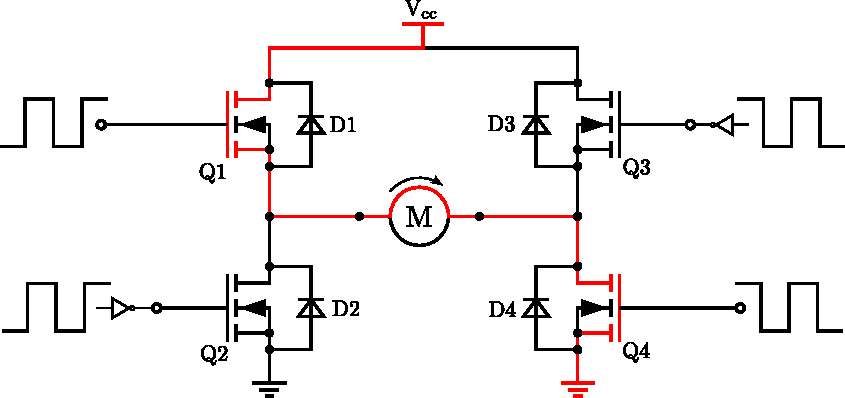
\includegraphics[scale=.53]{figures/HbridgeClockwise4Q.pdf}
  			\caption{Clockwise 4Q operation}
  			\label{HbridgeClokwise4Q}
  		\end{figure}
  	\end{minipage}
  	\hspace{0.03\linewidth}
  	\begin{minipage}{0.45\linewidth}
  		\begin{figure}[H]
  			\centering
  			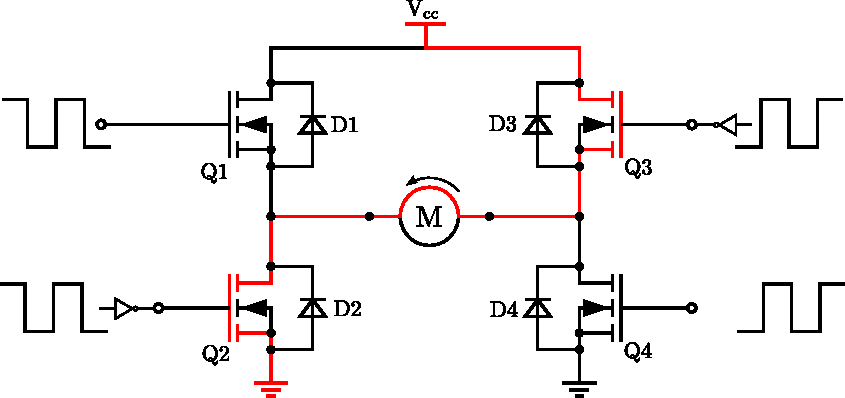
\includegraphics[scale=.53]{figures/HbridgeCounterClockwise4Q.pdf}
  			\caption{Counterclockwise 4Q operation}
  			\label{HbridgeCounterClokwise4Q}
  		\end{figure}
  	\end{minipage}
  \end{minipage}


\subsection{Brake Mode}
This mode of operation imposes the PWM signal on one side of the H-bridge, as seen on \figref{HbridgeClockwiseBrakeON} and \figref{HbridgeClockwiseBrakeOFF}. The PWM signal in collaboration with the NOT-gate shifts between Q1 and Q2, which provides the two current paths as shown. On \figref{HbridgeClockwiseBrakeON} the motor is driven by the supply, connected through Q1 and Q4. On \figref{HbridgeClockwiseBrakeOFF} the motor is short-circuited to ground through Q2 and Q4, which brakes on the motor.

  \begin{minipage}{\linewidth}
  	\centering
  	\begin{minipage}{0.45\linewidth}
  		\begin{figure}[H]
  			\centering
  			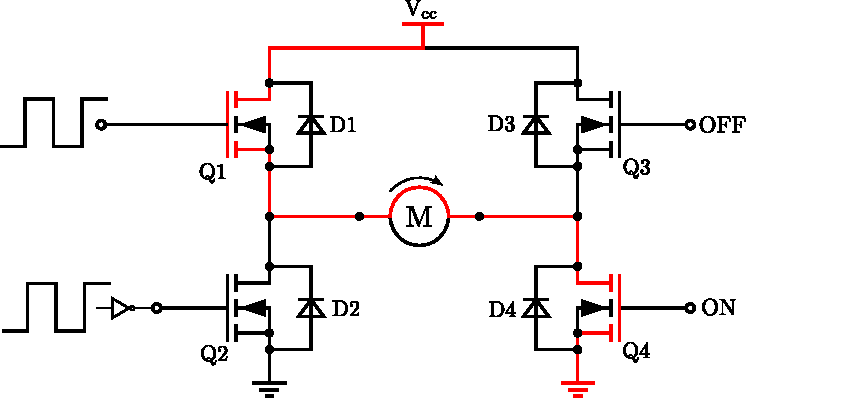
\includegraphics[scale=.6]{figures/HbridgeClockwiseBrakeON.pdf}
  			\caption{Clockwise brake operation in on-state}
  			\label{HbridgeClockwiseBrakeON}
  		\end{figure}
  	\end{minipage}
  	\hspace{0.03\linewidth}
  	\begin{minipage}{0.45\linewidth}
  		\begin{figure}[H]
  			\centering
  			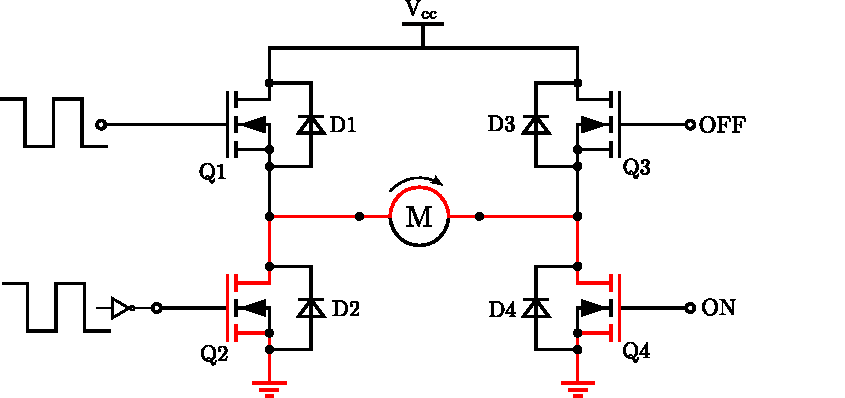
\includegraphics[scale=.6]{figures/HbridgeClockwiseBrakeOFF.pdf}
  			\caption{Clockwise brake operation in off-state}
  			\label{HbridgeClockwiseBrakeOFF}
  		\end{figure}
  	\end{minipage}
  \end{minipage}

\subsection{Double H-bridge Brake Mode}
Implemented on the vehicle is a double H-bridge, which is configured to run in brake mode as illustrated on \figref{DoubleHbridgeBrakeON} and \figref{DoubleHbridgeBrakeOFF}

\begin{figure}[H]
	\centering
	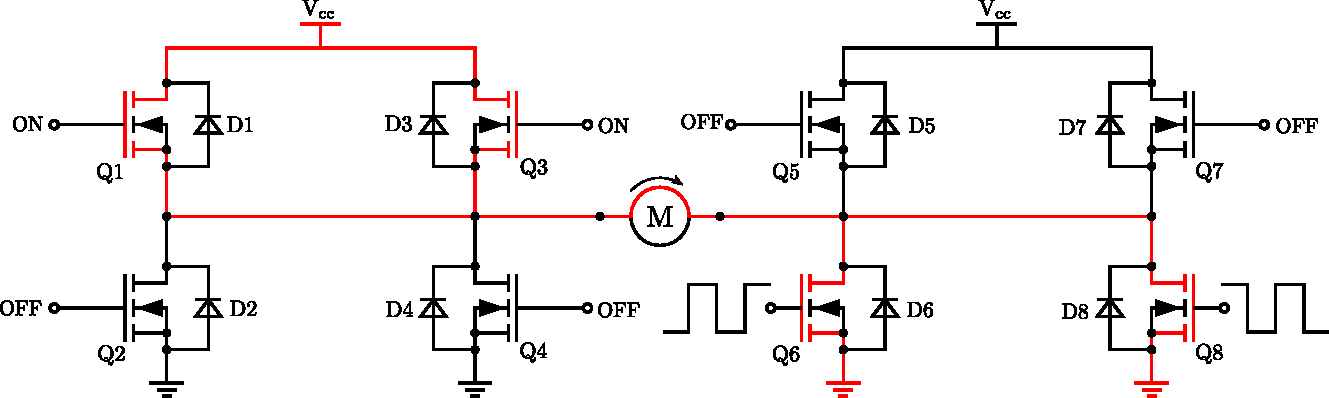
\includegraphics[scale=.6]{figures/DoubleHbridgeBrakeON.pdf}
	\caption{Double H-bridge brake operation in on-state}
	\label{DoubleHbridgeBrakeON}
\end{figure}

\begin{figure}[H]
	\centering
	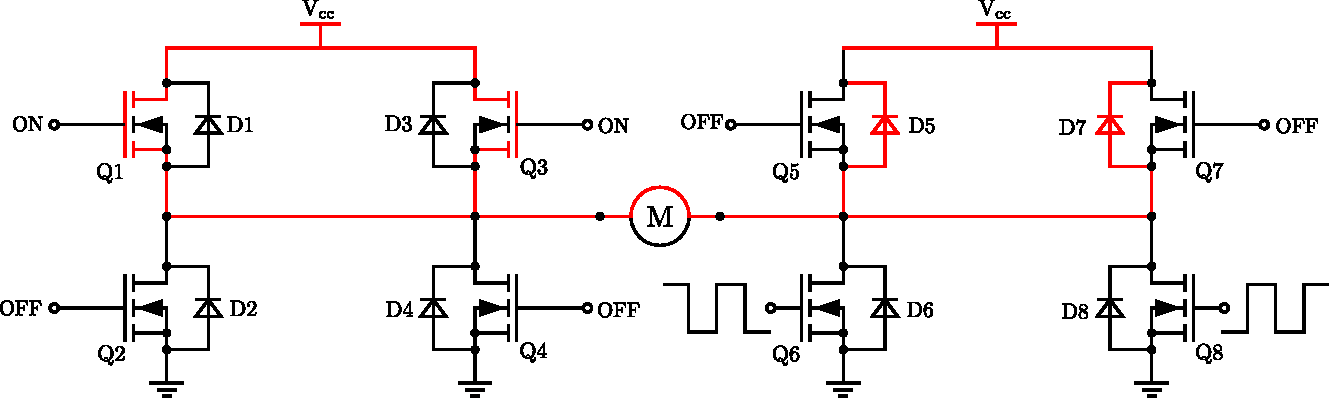
\includegraphics[scale=.6]{figures/DoubleHbridgeBrakeOFF.pdf}
	\caption{Double H-bridge brake operation in off-state}
	\label{DoubleHbridgeBrakeOFF}
\end{figure}

